
\chapter{Linear Algebra Applications}

This chapter covers the following ideas.  The purpose of this chapter is to show you a variety or applications of linear algebra, providing you with ample practice to polish up the skills learned in the arithmetic unit.  

\begin{enumerate}

\item Construct visualizations of matrices related to vector fields. Explain how eigenvalues and eigenvectors relate to vector fields.
\item Explain how to generalize the derivative to a matrix. Use this
  generalization to locate optimal values of a function using the second derivative test. Explain the role of eigenvalues and eigenvectors in the second derivative test.
\item Describe a Markov process. Explain what a steady-state solution is and how it relates to eigenvectors of the transition matrix.
\item Find the currents in an electrical system involving batteries and resistors, using both Gaussian elimination and Cramer's rule.
\item Find interpolating polynomials. Generalize this curve-fitting process to solve the least squares regression problem of fitting a line to a set of data.
\item Find bases for the column space, row space, and null space of a matrix and its transpose by row reducing $A$ and $A^T$. Use these bases to find the coordinates of vectors relative to the bases.

\end{enumerate}



%%% Local Variables: 
%%% mode: latex
%%% TeX-master: "../linear-algebra"
%%% End: 





\section{Vector Fields}



Vectors help us understand motion, forces, acceleration, and more. Imagine that you were a dust particle floating through the air.  Along the way, wind pushes you in various directions, sometimes causing you to swirl around, increasing your speed, or changing your direction. As you move through space, you encounter forces (vectors) pushing you around everywhere you go. This field of vectors provides an example of a vector field in space.  Magnetic fields, electrical fields, force fields, velocity fields, flow fields, and more are key ideas studied throughout the sciences. Meteorologists study air flow, physicists study magnetic and electric fields, and engineers study heat flow and fluid flow. In business, economists study the flow of money, which again results in studying vector fields. Pretty much every study of motion or change comes back to studying an underlying field of vectors.  In this section we will explore some simple two-dimensional vector fields arising from matrices, and then learn to physically observe the eigenvalues and eigenvectors from a plot of the vector field.  When studying more complicated vector fields, researchers use high dimensional calculus to simplify the complicated field to the vector fields we will study in this section. Eigenvalues and eigenvectors will play a major role.

Let's start with some notation. 
When you hear that $y$ is a function of $x$, you often write $y=f(x)$ to remind yourself that when you put in $x$ you get out $y$. 
For most of your lower level math courses, you have always thought of $x$ and $y$ as real numbers. 
In this case, the domain of the function (the $x$ values) is the set of real numbers which we denote with the symbol $\mathbb{R}$. \marginpar{$\mathbb{R}$ means all real numbers.} 
The potential $y$ values (the range) are also real numbers.  
If we want to pay attention to the domain and range of the function, we could write $f:D\to R$ \marginpar{$f:D\to R$ notation} where $D$ is the domain and $R$ is the range.  
For a function such as $y=f(x)$, where both $x$ and $y$ are real numbers (written $x\in \mathbb{R}$ and $y\in \mathbb{R}$), we could write $f:{\mathbb{R}}\to{\mathbb{R}}$. 
With this notation, we can generalize the concept of functions to allow us to input vectors and output vectors.  
If we want to input a 2D vector and get out a 3D vector, then we could write $f:{\mathbb{R}}^2\to{\mathbb{R}}^3$.  
We'll use the notation ${\mathbb{R}}^n$ to represent the set of $n$ dimensional vectors. 
Throughout this semester, we'll be studying functions of the form $f:{\mathbb{R}}^n\to {\mathbb{R}}^m$, in particular special functions called linear transformations which can often be represented by matrices.

A vector field is a function where you input a vector and output a vector of the same dimension. 
\marginpar{A vector field takes vectors of size $n$ to vectors of size $n$, $$f:{\mathbb{R}}^n\to{\mathbb{R}}^n.$$}
If $\vec x$ is a 2D vector, then a vector field is a function of the form $\vec F:{\mathbb{R}}^2\to {\mathbb{R}}^2$ (we put a vector above $\vec F$ because the output is a vector).  Think of the input as a point $(x,y)\in {\mathbb{R}}^2$, and the output as a vector $\vec F(x,y)\in {\mathbb{R}}^2$ whose base is placed at the point $(x,y)$.
Any square matrix represents a vector field.  If $A$ is a square matrix, then the function $\vec F(\vec x) = A\vec x$ tells that at the point $\vec x$ we should draw a vector $\vec F(\vec x)$. Let's look at an example and a graph.


\begin{example}
The matrix $\begin{bmatrix}2&1\\1&2\end{bmatrix}$ gives us the vector field $$\vec F(x,y)=\begin{bmatrix}2&1\\1&2\end{bmatrix}\begin{bmatrix}x\\y\end{bmatrix}=(2x+y,x+2y).$$ We input the point $(x,y)\in {\mathbb{R}}^2$ and get out the vector $(2x+y,x+2y)\in {\mathbb{R}}^2$.  For example, we compute $\vec F(1,0) = (2(1)+0,(1)+2(0)) = (2,1)$. To construct a graph of this fact, we place the vector $(2,1)$ in the plane with its base at $(1,0)$. To get a good view of what the vector fields does, we can pick an assortment of points in the plane, and then at each point we draw the vector obtained as output. The example below shows how to place the vectors corresponding to the 9 points with $x$ or $y$ coordinate $0, \pm 1$.  

\begin{center}
\begin{tikzpicture}
\node (A) {$\begin{array}{l|l}
(x,y) & \vec F(x,y)\\
\hline
(0,0) & (0,0) \\
(1,0) & (2,1) \\
(1,1) & (3,3) - \text{an eigenvalue is 3}\\
(0,1) & (1,2) \\
(-1,1) & (-1,1) - \text{an eigenvalue is 1}\\
(-1,0) & (-2,1) \\
(-1,-1) & (-3,-3) \\
(0,-1) & (-1,-2) \\
(1,-1) & (1,-1)
\end{array}$};
\node (vf) [right=of A] {
\includegraphics[height=2in]{02-Applications/support/vf21128points}};
\end{tikzpicture}
\end{center}


Notice that (1,1) is an eigenvector corresponding to the eigenvalue 3 because $A(1,1) = 3(1,1)$. 
Also, note that $(-1,1)$ is an eigenvector corresponding to the eigenvalue 1 because $A(-1,1)=(-1,1)$. 
These two eigenvectors represent the directions in which the vector field pushes objects radially outwards.   \marginpar{Eigenvectors tell you where vector fields push radially outwards.  Eigenvalues tell the strength and direction of the push.}
Anywhere along the line spanned by an eigenvector, the vector field pushes radially outward (as shown in the middle figure).  Starting on one side of an eigenvector requires that you stay on that side of the eigenvector forever. 
The eigenvalue tell you the strength of the push, which explains why the vectors in the $(1,1)$ direction are three times as long as the vectors in the $(-1,1)$ direction. 
The middle plot in Figure \ref{vf2112} includes two lines representing the eigenvector directions.

\begin{figure}[bth]
\begin{tikzpicture}[inner sep=0mm]
\node (A) 
{
\includegraphics[height=1.3in]{02-Applications/support/vf211225points}
};
\node (B) [right=of A] 
{
\includegraphics[height=1.3in]{02-Applications/support/vf2112com}
};
\node (C) [right=of B] 
{
\includegraphics[height=1.3in]{02-Applications/support/vf2112flow}
};
\end{tikzpicture}
\caption{\label{vf2112} Three views of the vector field $\vec F(x,y) =(2x+y,x+2y)$. The first plot shows the appropriate lengths.  The second plot includes two lines which come from the eigenvector directions. The third plot includes flow lines which describe the path of an object flowing through the vector field. Because flow is outward in all directions, this vector field is called a source.}
\end{figure}

When a computer draws a vector field, it creates hundreds of vectors, takes the longest vector and shrinks its length so that it won't cross any others, and then proportionally shrinks every other vector. This creates lots of tiny vectors which represent the directions (not magnitudes) of the vectors (see the last two plots in Figure \ref{vf2112}. You can think of a vector field as the flow of water, so that if you were to drop a particle into the field then it would follow the vectors (just as drift wood follows the flow of a river). These flow lines are represented in the last plot of Figure \ref{vf2112}.
\end{example} 

Figure \ref{vflots} contains multiple other examples. With example, the eigenvalues and eigenvectors provide valuable information to help understand how to draw flow lines in the graph.  Your job in the homework is to construct vector field plots by hand, find the corresponding eigenvalues and eigenvectors, and then from these construct flow lines (curves along which objects flow).


\begin{figure}
\begin{tikzpicture}[inner sep=0mm]
\node (B0) 
{
\includegraphics[width=1.3in]{02-Applications/support/vfsinkhand}
};
\node (A0) [left=of B0] 
{
\begin{tabular}{c}
Sink (inward flow)
\\ \hline
$A=
\begin{bmatrix}
 -2 & 2 \\
 1 & -2
\end{bmatrix}
$
\\
Eigenvalues: $-2-\sqrt{2},\sqrt{2}-2$
\\
Eigenvectors: $(-\sqrt{2} ,1), (\sqrt{2}, 1)$
\end{tabular}
};
\node (C0) [right=of B0] 
{
\includegraphics[width=1.3in]{02-Applications/support/vfsinkcom}
};

\node (B1) [below=of B0]
{
\includegraphics[width=1.3in]{02-Applications/support/vfrotationalhand}
};
\node (A1) [left=of B1] 
{
\begin{tabular}{c}
Rotational
\\ \hline
$A=
\begin{bmatrix}
 0 & -1 \\
 1 & 0
\end{bmatrix}
$
\\
Eigenvalues: $i,-i$
\\
Eigenvectors: $(i,1), (-1, 1)$
\end{tabular}
};
\node (C1) [right=of B1] 
{
\includegraphics[width=1.3in]{02-Applications/support/vfrotationalcom}
};

\node (B2) [below=of B1] 
{
\includegraphics[width=1.3in]{02-Applications/support/vfsaddlehand}
};
\node (A2) [left=of B2]
{
\begin{tabular}{c}
Saddle (both in and out)
\\ \hline
$A=
\begin{bmatrix}
 -1 & 4 \\
 2 & 3
\end{bmatrix}
$
\\
Eigenvalues: $5,-1$
\\
Eigenvectors: $(1,1), (-2, 1)$
\end{tabular}
};
\node (C2) [right=of B2] 
{
\includegraphics[width=1.3in]{02-Applications/support/vfsaddlecom}
};

\node (B3) [below=of B2] 
{
\includegraphics[width=1.3in]{02-Applications/support/vfspiralhand}
};
\node (A3) [left=of B3]
{
\begin{tabular}{c}
Outward Spiral
\\ \hline
$A=
\begin{bmatrix}
 1 & -1 \\
 1 & 1
\end{bmatrix}
$
\\
Eigenvalues: $1+i, 1-i$
\\
Eigenvectors: $(i ,1), (-i, 1)$
\end{tabular}
};
\node (C3) [right=of B3] 
{
\includegraphics[width=1.3in]{02-Applications/support/vfspiralcom}
};




\end{tikzpicture}
\caption{\label{vflots}
Different kinds of vector fields.  Every 2 by 2 matrix represents a vector field.  When the eigenvalues are real, the eigenvectors help determine direction of flow. Positive eigenvalues result in outward flow along the corresponding eigenvector. Negative eigenvalues result in inward flow. Pure imaginary eigenvalues yield rotational flow. When the eigenvalues involve both real and imaginary parts, the real part determines whether the flow is inward or outward, and the complex part results in rotation.
}
\end{figure}












\section{Kirchoff's Electrial Laws}
Gustav Kirchoff discovered two laws of electricity that pertain to the conservation of charge and energy. 
%In short, his two laws state that current in equals current out, and volts in equals volts out. 
To fully describe these laws, we must first discuss voltage, resistance, and current.  
Current is the flow of electricity; often you can compare it to the flow of water.  As a current passes across a conductor, it encounters resistance. 
Ohm's law states that the product of the resistance $R$ and current $I$ across a conductor equals a drop in voltage $V$, i.e. $RI=V$. \marginpar{\begin{center}Ohm's law: \\ Voltage = Resistance $\times$ Current$$V=RI$$\end{center}}
If the voltage remains constant, then a large resistance corresponds to a small current. 
A resistor is an object with high resistance which is placed in an electrical system to slow down the flow (current) of electricity. 
Resistors are measured in terms of ohms, and the larger the ohms, the smaller the current.  Figure \ref{ecir} illustrates two introductory electrical systems. 



\begin{figure}[htb]
\begin{center}
\begin{tabular}{cc}
\renewcommand{\myscale}{.3}
\begin{tikzpicture}[scale=\myscale,inner sep=1pt]
%\draw[help lines,step=1cm] (0,0) grid (12,6);

%Source - like a battery
\node[label=right:$E$] at (0,3) 
{{\begin{tikzpicture}[scale=\myscale]
%	\useasboundingbox (-.5,-3) rectangle (.5,3);
	\draw (0,0) circle (1cm);
	\draw (.3,.5) -- (-.3,.5);
	\draw (0,.2) -- (0,.8);
	\draw (.3,-.5) -- (-.3,-.5);
	\draw (0,1) -- (0,3);
	\draw (0,-1) -- (0,-3);
	\end{tikzpicture}
}};

%Resistor
\node[label=right:$R_2$] at (6,3) 
{{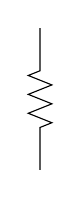
\begin{tikzpicture}[scale=\myscale]
%	\useasboundingbox (0,-3) rectangle (0,3);
	\draw (0,-3) -- ++(0,1.8) -- ++(.5,.2) 
		-- ++(-1,.4) -- ++(1,.4)
		-- ++(-1,.4) -- ++(1,.4)
		-- ++(-1,.4) -- ++(.5,.2)
		-- ++(0,1.8) ;
	\end{tikzpicture}
}};

%Resistor
\node[label=above:$R_1$] at (3,0) 
{{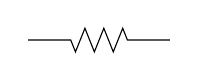
\begin{tikzpicture}[scale=\myscale,rotate=90]
%	\useasboundingbox (0,-3) rectangle (0,3);
	\draw (0,-3) -- ++(0,1.8) -- ++(.5,.2) 
		-- ++(-1,.4) -- ++(1,.4)
		-- ++(-1,.4) -- ++(1,.4)
		-- ++(-1,.4) -- ++(.5,.2)
		-- ++(0,1.8) ;
	\end{tikzpicture}
}};

%Resistor
\node[label=right:$R_3$] at (12,3) 
{{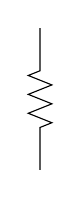
\begin{tikzpicture}[scale=\myscale,rotate=0]
%	\useasboundingbox (0,-3) rectangle (0,3);
	\draw (0,-3) -- ++(0,1.8) -- ++(.5,.2) 
		-- ++(-1,.4) -- ++(1,.4)
		-- ++(-1,.4) -- ++(1,.4)
		-- ++(-1,.4) -- ++(.5,.2)
		-- ++(0,1.8) ;
	\end{tikzpicture}
}};

%Straight Path
\node at (3,6) 
{{\begin{tikzpicture}[scale=\myscale,rotate=90]
	\draw (0,-3) -- (0,3);
	\end{tikzpicture}
}};

%Straight Path
\node at (9,6) 
{{\begin{tikzpicture}[scale=\myscale,rotate=90]
	\draw (0,-3) -- (0,3);
	\end{tikzpicture}
}};

%Straight Path
\node at (9,0) 
{{\begin{tikzpicture}[scale=\myscale,rotate=90]
	\draw (0,-3) -- (0,3);
	\end{tikzpicture}
}};


%Arrow to represent Current
\node[label=above:$i_1$] at (3,6) 
{{
\begin{tikzpicture}[scale=\myscale,rotate=-90]
%	\useasboundingbox (0,-.4) rectangle (0,.4);
	\filldraw (0,.4) -- (-.2,-.4) -- (0,-.3) -- (.2,-.4);
	\end{tikzpicture}
}};

%Arrow to represent Current
\node[label=right:$i_2$] at (6,5) 
{{
\begin{tikzpicture}[scale=\myscale,rotate=180]
%	\useasboundingbox (0,-.4) rectangle (0,.4);
	\filldraw (0,.4) -- (-.2,-.4) -- (0,-.3) -- (.2,-.4);
	\end{tikzpicture}
}};

%Arrow to represent Current
\node[label=above:$i_3$] at (9,6) 
{{
\begin{tikzpicture}[scale=\myscale,rotate=-90]
%	\useasboundingbox (0,-.4) rectangle (0,.4);
	\filldraw (0,.4) -- (-.2,-.4) -- (0,-.3) -- (.2,-.4);
	\end{tikzpicture}
}};

%Node
\node at (6,6) 
{{\begin{tikzpicture}[scale=\myscale,rotate=-90]
%	\useasboundingbox (0,-.4) rectangle (0,.4);
	\filldraw (0,0) circle (.15cm);
	\end{tikzpicture}
}};

%Node
\node at (6,0) 
{{\begin{tikzpicture}[scale=\myscale,rotate=-90]
%	\useasboundingbox (0,-.4) rectangle (0,.4);
	\filldraw (0,0) circle (.15cm);
	\end{tikzpicture}
}};

\end{tikzpicture}

&
\input{02-Applications/electric-circuit-3-loops}
\\
Two Loop System & Three Loop System
\end{tabular}\end{center}
\caption{Electrical Circuit Diagrams.}
\label{ecir}\end{figure}
In this diagram, wires meet at nodes (illustrated with a dot).  
Batteries and voltage sources (represented by 
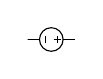
\begin{tikzpicture}[scale=.15,rotate=-90]
%	\useasboundingbox (-.5,-3) rectangle (.5,3);
	\clip (-1,-2) rectangle (1,2);
	\draw (0,0) circle (1cm);
	\draw (.3,.5) -- (-.3,.5);
	\draw (0,.2) -- (0,.8);
	\draw (.3,-.5) -- (-.3,-.5);
	\draw (0,1) -- (0,3);
	\draw (0,-1) -- (0,-3);
\end{tikzpicture}
or other symbols)
supply a voltage of $E$ volts.  At each node the current may change, so the arrows and letters $i$ represent the different currents in the electrical system. The electrical current on each wire may or may not follow the arrows drawn (a negative current means that the current flows opposite the arrow). Resistors are depicted with the symbol 	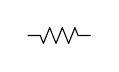
\begin{tikzpicture}[scale=.2,rotate=90]
%	\useasboundingbox (0,-3) rectangle (0,3);
	\clip (-.5,-2) rectangle (.5,2);
	\draw (0,-3) -- ++(0,1.8) -- ++(.5,.2) 
		-- ++(-1,.4) -- ++(1,.4)
		-- ++(-1,.4) -- ++(1,.4)
		-- ++(-1,.4) -- ++(.5,.2)
		-- ++(0,1.8) ;
	\end{tikzpicture}
, and the letter $R$ represents the ohms. 

Kirchoff discovered two laws which help us find the currents in a system, provided we know the voltage of any batteries and the resistance of any resistors. 
\begin{enumerate}
	\item Kirchoff's current law states that at every node, the current flowing in equals the current flowing out (at nodes, current in = current out). 
	\item Kirchoff's voltage law states that on any loop in the system, the directed sum of voltages supplied equals the directed sum of voltage drops (in loops, voltage in = voltage out). 
\end{enumerate}

Let's use Kirchoff's laws to generate some equations for the two loop system. 
\begin{enumerate}
	\item First we will examine Kirchoff's current law. 
	At the first node (top middle), current $i_1$ flows in while $i_2$ and $i_3$ flow out. 
	Kirchoff's current law states that 
	\marginpar{At each node, current in equals current out.}
	$$i_1=i_2+i_3$$ or $i_1-i_2-i_3=0$.  
	At the second node, both $i_2$ and $i_3$ are flowing in while $i_1$ flows out. 
	This means that $i_2+i_3=i_1$ or $-i_1+i_2+i_3=0$. 
	This second equation is the same as multiplying both sides of the first by $-1$ (so we say the 2nd equation depends on the first). 
	\item We now look at Kirchoff's voltage law. 
	Pick a loop and work your way around the loop in a clockwise fashion. 
	Each time you encounter a battery or resistor, include a term for the voltage supplied $E$ on the left side of an equation, and the voltage drop (resistance times current $Ri$) on the right. 
	If you encounter a battery or resistor as you work against the current, then times that term by $-1$. 
	
	The left loop has a battery with voltage $E$ (voltage in). 
	While moving along the wire containing $i_i$ we encounter a resistor with resistance $R_1$ which contributes a voltage drop of $R_1i_1$ volts. 
	Along $i_2$ we encounter $R_2$ for a drop of $R_2i_2$ volts. An equation for the first loop is 
	\marginpar{On loops, voltage in equals voltage out.}
	$$E=R_1i_1+R_2i_2.$$
	 
	On the right loop we encounter along current $i_3$ a resistor with resistance $R_3$ ohms.  
	While working our way against the arrow drawn on $i_2$, we encounter an $R_2$ ohm resistor (hence we have to put a negative sign in front of $R_2i_2$. \marginpar{Remember to change the sign when you cross a resistor while moving against the current.}
	There are no batteries on the second loop. The two resistors give us the equation $$0=-R_2 i_2 +R_3i_3.$$ 
\end{enumerate}
We can now write a system of equations involving the unknowns $i_1,i_2,i_3$, put it in matrix form, and then row reduce to solve
$$
\begin{array}{rl}
i_1-i_2-i_3&=0\\
-i_1+i_2+i_3&=0\\
R_1i_1+R_2i_2&=E\\
-R_2 i_2 +R_3i_3&=0
\end{array}
\xrightarrow{\text{matrix form}}
\begin{bmatrix}[ccc|c]
1&-1&-1&0\\
-1&1&1&0\\
R_1&R_2&0&E\\
0&-R_2&R_3&0
\end{bmatrix}
$$$$
\xrightarrow{\text{rref}}
\begin{bmatrix}[ccc|c]
 1 & 0 & 0 & \dfrac{E R_2+ E R_3}{R_1 R_2+R_1 R_3+R_2R_3} \\
 0 & 1 & 0 & \dfrac{E R_3}{R_1 R_2+R_1 R_3+R_2R_3} \\
 0 & 0 & 1 & \dfrac{E R_2}{R_1 R_2+R_1 R_3+R_2R_3} \\
 0 & 0 & 0 & 0
\end{bmatrix}.
$$
The reason we have a row of zeros at the bottom of our system is because the two rows corresponding to the nodes are linearly dependent.  
When we reduce the matrix, this row dependence results in a row of zeros.

A similar computation can be done for the three loop system. 
There are 6 unknown currents, 4 nodes, and 3 loops.  
This will give us 7 equations with 6 unknowns.  
The 4 equations from the nodes will again contribute rows which are linearly dependent, which means you can always ignore an equation from one of the nodes. \marginpar{If there are $n$ nodes in a problem, you only need to consider $n-1$ of them, as the $n$ equations are dependent.}
In electrical network problem, row reduction will always give a unique solution. 
In the homework, you are asked to setup systems of equations for various electrical systems, and then solve them. 


\begin{example} \label{electrical example}Let's look at an example which involves numbers.  Suppose $E=12$ (a 12 volt battery) and the resistors have $R_1=2, R_2=R_3=4$ ohms. The top node gives the equation $i_1=i_2+i_3$ (remember flow in equals flow out). We'll skip the bottom node, as it contributes another row which is dependent on the first.  The left loop gives the equation $12 = 2i_1+4i_2$, while the right loop gives the equation $0=-4r_2+4r_3$.  We write this in matrix form
$$
\begin{array}{rl}
i_1-i_2-i_3&=0\\
2i_1+4i_2&=12\\
-4 i_2 +4i_3&=0
\end{array}
\xrightarrow{\text{matrix form}}
\begin{bmatrix}[ccc|c]
1&-1&-1&0\\
2&4&0&12\\
0&-4&4&0
\end{bmatrix}
\xrightarrow{\text{rref}}
\begin{bmatrix}[ccc|c]
 1 & 0 & 0 & 3\\
 0 & 1 & 0 & 3/2\\
 0 & 0 & 1 & 3/2
\end{bmatrix}
$$
which tells us the currents are $i_1=3$, $i_2=3/2$, and $i_3=3/2$.
\end{example}






\subsection{Cramer's Rule}
Cramer's rule is a theoretical tool which gives the solution to any linear system $A\vec x = \vec b$ with $n$ equations and $n$ unknowns, provided that there is a unique solution.  
Let $D=\det(A)$. 
Let $D_i$ be the determinant of the matrix formed by replacing the $i$th column of $A$ with $\vec b$.  
Then Cramer's rule states that $$x_1 = \frac{D_1}{D},x_2 = \frac{D_2}{D},\ldots, x_n = \frac{D_n}{D}.$$ 
We may prove it in class with pictures which connect determinants to area (eventually I'll add this to an appendix)\note{appendix problem}. 
This method of solving a system of equations is quickly doable for 2 by 2 and 3 by 3 systems, but becomes computationally inefficient beyond (as computing determinants is time consuming and numerically unstable on large matrices). 
\marginpar{Cramer's rule works great on 2 by 2 and 3 by 3 systems, where determinants are easy to compute.}
For large systems, it is better to use Gaussian elimination. 
However, Cramer's rule is a powerful theoretical tool, and can simplify symbolic computations for small systems. Let's look at a few examples.

\begin{example}
Let's solve $
\begin {bmatrix} 1&2&0\\-2&0&1\\0&3&-2\end {bmatrix} 
\begin {bmatrix} x_1\\x_2\\x_3\end {bmatrix} 
=  \begin{bmatrix} 2\\-2\\1\end {bmatrix}
$ using Cramer's rule.  
We compute the determinant of the coefficient matrix first to obtain
$$D=\begin{vmatrix} 1&2&0\\-2&0&1\\0&3&-2\end {vmatrix} = -11.$$ Next we replace each column of the coefficient matrix with the right column of our augmented system and compute the three determinants to obtain
$$
\begin{vmatrix} 
\tikz \draw node[fill=pink,inner sep=0cm]{$\cl{2\\-2\\1}$};
& \tikz \draw node[inner sep=0cm]{$\cl{2\\0\\3}$};
&\tikz\draw node[inner sep=0cm]{$\cl{0\\1\\-2}$};
\end {vmatrix}  
 =-12,
\begin{vmatrix} 
\tikz \draw node[inner sep=0cm]{$\cl{1\\-2\\0}$};
& \tikz \draw node[fill=pink,inner sep=0cm]{$\cl{2\\-2\\1}$};
&\tikz\draw node[inner sep=0cm]{$\cl{0\\1\\-2}$};
\end {vmatrix}  
=-5, 
\begin{vmatrix} 
\tikz \draw node[inner sep=0cm]{$\cl{1\\-2\\0}$};
& \tikz \draw node[inner sep=0cm]{$\cl{2\\0\\3}$};
&\tikz \draw node[fill=pink,inner sep=0cm]{$\cl{2\\-2\\1}$};
\end {vmatrix}  
=-2 .$$
Cramer's rule requires that we divide each of these determinants by the original determinant, giving the solution $x_1=12/11, x_2 = 5/11, x_3 = 2/11$.  Using Gaussian Elimination, we obtain the same solution 
$$ \begin {bmatrix}[ccc|c] 1&2&0&2\\-2&0&1&-2\\0&3&-2&1\end {bmatrix}\xrightarrow{\text{rref}}
\begin {bmatrix}[cccc] 1&0&0&12/11
\\0&1&0&5/11\\0&0&1&2/11\end {bmatrix} 
, $$
however the arithmetic involved in keeping track of fractions or really large integers becomes much more difficult by hand without Cramer's rule.
\end{example}

\begin{example}
Consider the electrical system in Example \ref{electrical example} where $E=12$, $R_1=2$, and $R_2=R_3=4$. 
The corresponding augmented matrix we used to solve this system was 
$$
\begin{bmatrix}[ccc|c]
1&-1&-1&0\\
2&4&0&12\\
0&-4&4&0
\end{bmatrix}, 
A=
\begin{bmatrix}1&-1&-1\\2&4&0\\0&-4&4\end{bmatrix}, 
\vec b=\begin{bmatrix}
0\\
12\\
0
\end{bmatrix},D=\begin{vmatrix} 1&-1&-1\\2&4&0\\0&-4&4 \end {vmatrix} =32. 
$$ 
We now replace each column with $\vec b$ and compute the determinant of the corresponding matrix (remember to cofactor along the column which contains $0,12,0$ to do this quickly)
$$ 
D_1=\begin{vmatrix} 0&-1&-1\\12&4&0\\0&-4&4 \end {vmatrix} =96,
D_2=\begin{vmatrix} 1&0&-1\\2&12&0\\0&0&4 \end {vmatrix} =48, 
D_3=\begin{vmatrix} 1&-1&0\\2&4&12\\0&-4&0 \end {vmatrix} =48. 
$$
Dividing each of these by the determinant of the original matrix gives the solution $i_1 = 96/32 = 3$, $i_2=i_3=48/32 = 3/2$, which matches the solution we found using row reduction in the previous section. 
\end{example}



















\section{Fitting Curves to Data}
\subsection{Interpolating Polynomials}
Through any two points (with different $x$ values) there is a unique line of the form $y=mx+b$. If you know two points, then you can use them to find the values $m$ and $b$.  
Through any 3 points (with different $x$ values) there is a unique parabola of the form $y=ax^2+bx+c$, and you can use the 3 points to find the values $a,b,c$.  
\marginpar{Through $n+1$ points (with different $x$ values), there is a unique polynomial of degree $n$ which passes through those points.}
As you increase the number of points, there is still a unique polynomial (called an interpolating polynomial) with degree one less than the number of points, and you can use the points to find the coefficients of the polynomial. 
In this section we will illustrate how to find interpolating polynomials, and show how the solution requires solving a linear system. Cramer's rule or Gaussian elimination will give us the solution. 

To organize our work, let's first standardize the notation.  
Rather than writing $y=mx+b$, let's write $y=a_0+a_1 x$ (where $a_0=b$ and $a_1=m$). 
For a parabola, let's write $\ds y=a_0 + a_1 x+ a_2 x^2 = \sum_{k=0}^{2} a_k x^k$. 
We can now write any polynomial in the form 
\marginpar{Standardizing the notation makes a problem easier to generalize.}  $$\ds y = a_0 + a_1 x+ \cdots + a_n x^n = \sum_{k=0}^n a_k x^k.$$ 
By standardizing the coefficients, we can use summation notation to express a polynomial of any degree by changing the $n$ on the top of the summation sign. 
Now that our notation is organized, let's use it to find a polynomial through 3 points.

\begin{example}\note{add in a graph}
Let's find a parabola through the three points $(0, 1), (2, 3), (4, 7)$.  The polynomial is $y=a_0 +a_1 x+a_2 x^2$ and our job is to find the three constants $a_0, a_1, a_2$.  Since we have three points, we put these points into the equation to obtain the three equations
$$
a_{{0}}=1 \quad \quad 
a_{{0}}+2\,a_{{1}}+4\,a_{{2}}=3 \quad \quad 
a_{{0}}+4\,a_{{1}}+16\,a_{{2}}=7
$$
This is a linear system with 3 equations and 3 unknowns.  We now write the system in matrix form and reduce it
$$
\begin{bmatrix}[ccc|c] 
1&0&0&1\\
1&2&4&3\\
1&4&16&7
\end {bmatrix}
\xrightarrow{\text{rref}}
\begin{bmatrix}[ccc|c]
1&0&0&1\\
0&1&0&1/2\\
0&0&1&1/4
\end {bmatrix} 
.$$
The reduced row echelon form tells us that the coefficients are $a_0 = 1, a_1= 1/2, a_2=1/4$, which means our parabola is $y=1+\frac12 x+ \frac 14 x^2$. Cramer's rule gives $D=16, D_1=16, D_2=8, D_3=4$, and so $a_0 = 16/16=1, a_1=8/16=1/2, a_2=4/16=1/4$, the same as with Gaussian elimination. 

\marginpar{Check your work by plugging the points back into your solution.}
Once you have obtained your interpolating polynomial, you can always check your work by putting the points back into your new equation. When $x=0$ we have $y=1+0+0=1$, when $x=2$ we have $1+1+1=3$, and when $x=4$ we have $1+2+4=7$, which means the parabola passes through the three points (0,1), (2,3), and (4,7) as needed.  
\end{example}

In the example above, notice that powers of $x$ appear as the coefficients of our coefficient matrix, and we augment that matrix by the $y$ values. This is the general pattern for finding an interpolating polynomial. The diagram below shows the general method for finding an interpolating polynomial through three points.
\begin{center}
\begin{tabular}{c}
$(x_1,y_1),(x_2,y_2),(x_3,y_3)$ \\
 $
\begin{bmatrix}[ccc|c] 
x_1^0=1&x_1^1&x_1^2&y_1\\
1&x_2^1&x_2^2&y_2\\
1&x_3^1&x_3^2&y_3
\end {bmatrix}
\xrightarrow{\text{rref}}
\begin{bmatrix}[ccc|c]
1&0&0&a_0\\
0&1&0&a_1\\
0&0&1&a_2
\end {bmatrix} 
$
\\
 $y=a_0+a_1x+a_2x^2$
\end{tabular}
\end{center}
Finding an interpolating polynomial through 4 points is very similar, you just have to add one more row and column to the matrix and repeat the process.
\begin{center}
\begin{tabular}{c}
$(x_1,y_1),(x_2,y_2),(x_3,y_3),(x_4,y_4)$\\
$
\begin{bmatrix}[cccc|c] 
1&x_1^1&x_1^2&x_1^3&y_1\\
1&x_2^1&x_2^2&x_2^3&y_2\\
1&x_3^1&x_3^2&x_3^3&y_3\\
1&x_4^1&x_4^2&x_4^3&y_4
\end {bmatrix}
\xrightarrow{\text{rref}}
\begin{bmatrix}[cccc|c]
1&0&0&0&a_0\\
0&1&0&0&a_1\\
0&0&1&0&a_2\\
0&0&0&1&a_3
\end {bmatrix} 
$\\
$y=a_0+a_1x+a_2x^2+a_3x^3$
\end{tabular}
\end{center}
This pattern generalizes to all dimensions (and the corresponding algorithm is coded into spread sheet programs such as Microsoft Excel and OpenOffice Calc). Remember that the $x$ values must be different (a function requires only one output for each input). Once you have obtained your solution, remember that you can easily check if your solution is correct by plugging the points into your equation. 





















\subsection{Least Squares Regression}
Interpolating polynomials give a polynomial which passes through every point in a set of data. 
While they pass through every point in a set of data, the more points the polynomial must pass through, the more the polynomial may have to make large oscillations in order to pass through each point.  
Often we just need a simple line or parabola that passes near the points and gives a good approximation of a trend. 
Here's an example that saved me tons of money when buying a minivan. 
When I needed to purchase a minivan for my expanding family, I gathered mileage and price data for about 40 cars from the internet. 
I plotted this data and discovered an almost linear downward trend (as mileage increased, the price dropped).  
I created a line to predict the price of a car based on mileage.  
I then used this data to talk the dealer into dropping the price of the car I wanted by over \$1000. 
\note{I need to find this data on our computer and put a graph here}
Finding an equation of this line, called the least squares regression line, is the content of this section. 
How do you find a line that is ``closest'' to passing through 3 or more points?  
The least squares regression line is used to find trends in many branches of science, in addition to haggling for lower prices when buying a car. Let's introduce the idea with an example. 

\begin{example}\label{regression1ex}
Let's find a line that is closest to passing through the three points $(0,1)$, $(2,3)$, and $(4,6)$.  Since the points are not collinear, there is not a line through all three.  Suppose for a moment that there were a line of the form $y=mx+b=a_0+a_1x$ (let's use our standardized notation) that did pass through the points. Pluggin our 3 points into the equation $a_0+a_1x=y$ gives the system of equations 
$$\begin{cases}a_0=1\\a_0+2a_1=3\\a_0+4a_1=6\end{cases}
\xrightarrow{\text{augmented matrix}}
\begin{bmatrix}[cc|c]1&0&1\\1&2&3\\1&4&6\end{bmatrix}
\xrightarrow{\text{matrix eqn}}
\begin{bmatrix}1&0\\1&2\\1&4\end{bmatrix}
\begin{bmatrix}a_0\\a_1\end{bmatrix}
=\begin{bmatrix}3\\1\\6\end{bmatrix}.
$$
Notice that the system can be written in matrix form $A\vec x = \vec b$ where $A$ contains a column of 1's and $x$ values, and $\vec b$ is a column of $y$ values. 
If you try to reduce this matrix, you will discover the system is inconsistent (has no solution) which should not be a surprise since there is no line which passes through these three points. 
Notice that there are more equations (3 equations) than variables ($a_0$ and $a_1$), which means the system is over determined.
\marginpar{Recall that if a system has more equations than variables, we say the system is over determined.} 

While there is no solution, can we still use our matrix equation to find a solution? 
Is there a way to reduce the number of rows in our system, so that the resulting system has only 2 rows? 
If we multiply on the left by a 2 by 3 matrix, we would obtain a system with 2 rows instead of 3, and the rows of the new matrix would be linear combinations of the rows of our original matrix.  
The only 2 by 3 matrix in this problem is the transpose of A.  
So let's multiply both sides of the matrix equation by the transpose of A, and see what happens:
$$A = \begin{bmatrix}1&0\\1&2\\1&4\end{bmatrix}, 
A^T = \begin{bmatrix}1&1&1\\0&2&4\end{bmatrix},$$$$ 
A^T A =\begin{bmatrix}1&1&1\\0&2&4\end{bmatrix}\begin{bmatrix}1&0\\1&2\\1&4\end{bmatrix}= \begin{bmatrix}3&6\\6&20\end{bmatrix}, 
A^T\vec b =  \begin{bmatrix}1&1&1\\0&2&4\end{bmatrix}\begin{bmatrix}1\\3\\6\end{bmatrix} = \begin{bmatrix}10\\30\end{bmatrix}.
$$
\marginpar{Multiply both sides by $A^T$, the transpose of $A$, to obtain a system that has a solution.}
Multiplying both sides of the equation $A\vec x = \vec b$ on the left by $A^T$ gives us the equation 
$A^T A \vec x = A^T\vec b$, or 
$$\begin{bmatrix}3&6\\6&20\end{bmatrix} \begin{bmatrix}a_0\\a_1\end{bmatrix}=\begin{bmatrix}10\\30\end{bmatrix}.$$ 
This is a system of 2 equations with 2 unknowns, and it has a unique solution.  
Reducing $\begin{bmatrix}[cc|c]3&6&10\\6&20&30\end{bmatrix}$ to $\begin{bmatrix}[cc|c]1&0&5/6\\0&1&5/4\end{bmatrix}$ means the solution is $y=\frac{5}{6}+\frac{5}{4}x.$  
We will see exactly why this works later in this chapter, when we start looking at the columns of our matrix as a basis for a vector space and asking questions about linear combinations, spans, and projections.   
For now, let's just use the transpose to solve least squares regression problems. I'm hoping you want to know why this works, and I promise you will get an answer. 
\end{example}

In general, a least squares regression problem requires the following:
\begin{enumerate}
	\item Assume the form of a solution, such as $y=a_0+a_1x$ for a line. 
	\item Plug in values to get a matrix equation $A\vec x=\vec b$. 
	\item Multiply both sides by $A^T$.
	\item Solve the simplified system (elimination, Cramer's rule, or an inverse). 
\end{enumerate}
When trying to find a least squares regression line, the simplified systems will be a 2 by 2 system so Cramer's rule provides an extremely quick solution. 

\begin{example}
Let's find the least squares regression line which passes nearest the four points $(0,0)$, $(-1,2)$, $(-2,4)$, and $(0,-1)$. We are after an equation of the form $y=a_0+a_1x$.  The four points give the equations $a_0=0, a_0-a_1=2, a_0-2a_1=4, a_0=-1$. In matrix form we write 
$$
\begin{bmatrix}
1&0\\
1&-1\\
1&-2\\
1&0
\end{bmatrix}
\begin{bmatrix}
a_0\\
a_1
\end{bmatrix}
=
\begin{bmatrix}
0\\
2\\
4\\
-1
\end{bmatrix}
,
A=
\begin{bmatrix}
1&0\\
1&-1\\
1&-2\\
1&0
\end{bmatrix}, 
\vec b = 
\begin{bmatrix}
0\\
2\\
4\\
-1
\end{bmatrix}, 
$$
$$
A^T=
\begin{bmatrix}
1&1&1&1\\
0&-1&-2&0
\end{bmatrix}, 
A^TA = 
\begin{bmatrix}
4&-3\\
-3&5
\end{bmatrix}, 
A^T\vec b =
\begin{bmatrix}
5\\
-10
\end{bmatrix}. 
$$
We now need to solve the matrix equation 
$
\begin{bmatrix}
4&-3\\
-3&5
\end{bmatrix}\begin{bmatrix}
a_0\\
a_1
\end{bmatrix}
=
\begin{bmatrix}
5\\
-10
\end{bmatrix}. 
$
Cramer's rule gives the solution as
$$
a_0
=\frac{\begin{vmatrix}
5&-3\\
-10&5
\end{vmatrix}}{\begin{vmatrix}
4&-3\\
-3&5
\end{vmatrix}}
=\dfrac{-5}{11}
, \quad\quad\quad
a_1
=\frac{\begin{vmatrix}
4&5\\
-3&-10
\end{vmatrix}}{\begin{vmatrix}
4&-3\\
-3&5
\end{vmatrix}}
=\dfrac{-25}{11}
.$$
The least square regression line is $y=-\frac{5}{11}-\frac{25}{11}x$.
\end{example}
















\subsection{A Quick 2 by 2 Inverse}
Finding the least square regression line requires solving the system $A^TA\vec x = A^T \vec b$ for $\vec x$. Symbolically we can solve this system by multiplying both sides on the left by $(A^TA)^{-1}$ (this inverse will exist), giving the solution 
$$\vec x = \begin{bmatrix}a_0\\a_1\end{bmatrix}= (A^TA)^{-1}A^T \vec b.$$ 

For 2 by 2 matrices, there is quick way to find the inverse. 
To find the inverse of a 2 by 2 matrix $A=\begin{bmatrix}a&b\\c&d\end{bmatrix}$, we need to reduce $\begin{bmatrix}[cc|c]a&b&1\\c&d&0\end{bmatrix}$ to find the first column of the inverse, and $\begin{bmatrix}[cc|c]a&b&0\\c&d&1\end{bmatrix}$ to find the second column.  
Cramer's rule gives the formula 
\marginpar{To find the inverse of a 2 by 2, 
\begin{enumerate}
	\item switch the diagonals, 
	\item change the sign on the off diagonals, and 
	\item divide by the determinant.
\end{enumerate}
}
$$A^{-1}=
\begin{bmatrix}
\begin{vmatrix}1&b\\0&d\end{vmatrix}/|A|&\begin{vmatrix}0&b\\1&d\end{vmatrix}/|A|\\ \\
\begin{vmatrix}a&1\\c&0\end{vmatrix}/|A|&\begin{vmatrix}a&0\\c&1\end{vmatrix}/|A|\end{bmatrix} 
= \frac{1}{|A|}
\begin{bmatrix}d&-b\\-c&a\end{bmatrix}
$$
To find the inverse of a 2 by 2 matrix, just interchange the diagonal entries, change the sign on the others, and divide by the determinant.

\begin{example}
Let's repeat the introductory example (\ref{regression1ex}) from the last section by using an inverse to find the line closest to passing through the three points $(0,1)$, $(2,3)$, and $(4,6)$. The matrix equation and relevant matrices are
$$\begin{bmatrix}1&0\\1&2\\1&4\end{bmatrix}
\begin{bmatrix}a_0\\a_1\end{bmatrix}
=\begin{bmatrix}3\\1\\6\end{bmatrix},
A = \begin{bmatrix}1&0\\1&2\\1&4\end{bmatrix},
\vec b = \begin{bmatrix}1\\3\\6\end{bmatrix}, $$$$
A^T= \begin{bmatrix}1&1&1\\0&2&4\end{bmatrix}, 
A^T A= \begin{bmatrix}3&6\\6&20\end{bmatrix}, 
A^T\vec b = \begin{bmatrix}10\\30\end{bmatrix}.
$$
The inverse of $(A^TA)$ is $\ds\frac{1}{60-36}\begin{bmatrix}20&-6\\-6&3\end{bmatrix}$, which means our solution is 
$$
\begin{bmatrix}a_0\\a_1\end{bmatrix} 
= (A^TA)^{-1}A^T b 
= \ds\frac{1}{24}\begin{bmatrix}20&-6\\-6&3\end{bmatrix}\begin{bmatrix}10\\30\end{bmatrix}
= \ds\frac{1}{24}\begin{bmatrix}20\\30\end{bmatrix}  
= \begin{bmatrix}5/6\\5/4\end{bmatrix}. 
$$
We of course obtained the same solution $y=\frac{5}{6}+\frac{5}{4}x$.
\end{example}


One advantage of using an inverse to solve a least square regression problem is that the product $W=(A^TA)^{-1}A^T$ can be computed once, and then solutions to similar least squares regression problems are found by the simple product $\vec x=W\vec b$. 
A different set of data points where the $x$ values remain the same but the $y$ values change can then be solved by just changing $\vec b$ and using the same results as before. 

\begin{example}
Let's find the least square regression line for the two data sets 
\begin{enumerate}
	\item $(0,2)$, $(2,1)$, and $(4,3)$
	\item $(0,6)$, $(2,3)$, and $(4,-1)$
\end{enumerate}
Notice that both of the data sets have the same $x$ values as the previous example.  Hence we can still use 
$$
A = \begin{bmatrix}1&0\\1&2\\1&4\end{bmatrix},
A^T= \begin{bmatrix}1&1&1\\0&2&4\end{bmatrix}, 
A^T A= \begin{bmatrix}3&6\\6&20\end{bmatrix}, 
(A^TA)^{-1}=\ds\frac{1}{24}\begin{bmatrix}20&-6\\-6&3\end{bmatrix}.
$$ 
The change occurred with the $y$ values, which means that $\vec b$ changed for each problem.  Before solving either, we compute 
$$W=(A^TA)^{-1}A^T 
= \ds\frac{1}{24}\begin{bmatrix}20&-6\\-6&3\end{bmatrix}\begin{bmatrix}1&1&1\\0&2&4\end{bmatrix}
= \ds\frac{1}{24}\begin{bmatrix}20&8&-4\\-6&0&6\end{bmatrix}
$$
We can now solve both problems rapidly, by multiplying $W$ and $\vec b$.
\begin{enumerate}
	\item The $y$ values are $2,1,3$, so we compute
$$\frac{1}{24}\begin{bmatrix}20&8&-4\\-6&0&6\end{bmatrix} \begin{bmatrix}2\\1\\3\end{bmatrix}
= \frac{1}{24}\begin{bmatrix}36\\6\end{bmatrix}
$$ which means that our line is (after simplifying fractions) $y=\frac{3}{2}+\frac{1}{4}x$.
	\item The $y$ values are $6,3,-1$, so we compute
$$\frac{1}{24}\begin{bmatrix}20&8&-4\\-6&0&6\end{bmatrix} \begin{bmatrix}6\\3\\-1\end{bmatrix}
= \frac{1}{24}\begin{bmatrix}148\\-42\end{bmatrix}
$$ which means that our line is (after simplifying fractions) $y=\frac{37}{6}-\frac{7}{4}x$.
\end{enumerate}
\end{example}

Least squares regression is not limited to just finding a best fit line.  We can use the same ideas to find a best fitting parabola through many points.  We would start by assuming the data fit a parabola $y=a_0+a_1x+a_2x^2$, plug in the $x$ and $y$ values to obtain a linear system with 3 unknowns, write the system in matrix form (the columns of the matrix would involve 1's, $x$ values, and $x^2$ values), multiply both sides by the transpose to obtain a 3 by 3 matrix, and then solve the system.  Most spread sheet programs have this feature built in for any size polynomial you choose.









\section{The Second Derivative Test}

In this section, we'll explore how eigenvalues and eigenvectors of a matrix are the key tool needed to generalize the second derivative test from first semester calculus to all dimensions. The key application is that eigenvalues tell you about concavity of a function in the eigenvector directions.  If all eigenvalues are negative, then a function is concave downwards in all directions, which means that a critical point must correspond to a maximum.    

Let's start with a review from first semester calculus. 
If a function $y=f(x)$ has a relative extreme value at $x=c$, then $f^\prime(c)=0$ or the derivative is undefined. 
The places where the derivative is either zero or undefined are called critical values of the function. 
The first derivative test allows you to check the value of the derivative on both sides of the critical value and then interpret whether that point is a maximum or minimum using increasing/decreasing arguments.  
The second derivative test requires you to compute the second derivative at $x=c$ and then make an observation. 
If $f''(c)>0$ (the function is concave upwards), then the function has a minimum at $x=c$. 
If $f''(c)<0$ (the function is concave downwards), then the function has a maximum at $x=c$. 
If $f''(c)=0$, then the second derivative test fails. 
\note{pictures would be good}

\begin{example}
The function $f(x) = x^3-3x$ has derivatives $f^\prime = 3x^2-3$ and $f^{\prime\prime}=6x$.  The first derivative is zero when $3(x^2-1)=3(x-1)(x+1)=0$, or $x=\pm 1$.  
The second derivative at $x=1$ is $f''(1)=6$ (concave upwards), so there is a minimum at $x=1$.  
The second derivative at $x=-1$ is $f''(-1)=-6$ (concave downwards), so there is a maximum at that point. This is all illustrated to the right.
\marginpar{\includegraphics[width=\marginparwidth]{02-Applications/support/sage0.png}}
\end{example}

\subsection{Partial Derivatives}

Before extending the second derivative test to all dimensions, we have to talk about taking derivatives.
If a function has more than one input variable, say $f(x,y)=9-x^2+3y$ which has 2 input variables, then we have to take multiple derivatives, one with respect to each variable.  
These derivatives (called partial derivatives) are found by holding all variables constant except the one you want the derivative with respect to, and then just computing a normal derivative.
For the function $f(x,y)$, we define the partial derivative of $f$ with respect to $x$ as 
$$\ds f_x(x,y)=f_x = \frac{\partial f}{\partial x}= \lim_{h\to 0}\frac{f(x+h,y)-f(x,y)}{h},$$
and the partial derivative of $f$ with respect to $y$ as 
$$\ds f_y(x,y)=f_y =\frac{\partial f}{\partial y}= \lim_{k\to 0}\frac{f(x,y+k)-f(x,y)}{k}.$$
Notice that $f_x$ computes a limit as $y$ is held constant and we vary $x$. 

\begin{example}
For $f(x,y)=3x^2+4xy+\cos(xy)+y^3$, we obtain $f_x=6x+4y-y\sin(xy)+0$ and $f_y=0+4x-x\sin(xy)+3y^2$. 
Partial derivatives are found by holding all other variables constant, and then differentiating with respect to the variable in question.
\end{example}

\subsection{The Derivative}
The derivative of a function $\vec f:\mathbb{R}^n\to\mathbb{R}^m$ is an $m\times n$ matrix written $D\vec f(\vec x)$, where the columns of the matrix are the partial derivatives of the function with respect to an input variable (the first column is the partial derivative with respect to the first variable, and so on). Some people call this derivative the ``total'' derivative instead of the derivative, to emphasize that the ``total'' derivative combines the ``partial'' derivatives into a matrix. Some examples of functions and their derivative are in Table \ref{dertable}. Remember that each input variable corresponds to a column of the matrix.   
\begin{table}[htb]
\begin{center}
\begin{tabular}{|l|l|}
\hline
Function&Derivative\\ \hline
{$f(x)=x^2$}& {$Df(x) = \begin{bmatrix}2x\end{bmatrix} $}\\ \hline
{$\vec r(t) = \left<3\cos(t),2\sin(t)\right>$}&  {$D\vec r(t) = \begin{bmatrix}-3\sin t\\ 2\cos t\end{bmatrix} $}\\ \hline
{$\vec r(t) = \left<\cos(t),\sin(t),t\right>$}&  {$D\vec r(t) = \begin{bmatrix}-\sin t \\ \cos t \\ 1\end{bmatrix} $}\\ \hline
{$f(x,y)=9-x^2-y^2$}&  {$Df(x,y) = \begin{bmatrix}-2x & -2y\end{bmatrix} $}\\ \hline
{$f(x,y,z)=x^2+y+xz^2$}&  {$Df(x,y,z) = \begin{bmatrix}2x+z^2 & 1 &2xz\end{bmatrix} $}\\ \hline
{$\vec F(x,y)=\left<-y,x\right>$}&  {$D\vec F(x,y) = \begin{bmatrix}0&-1\\ 1&0\end{bmatrix} $}\\ \hline
{$\vec F(r,\theta,z)=\left<r\cos\theta,r\sin\theta,z\right>$}&  {$D\vec F(r,\theta,z) = 
\begin{bmatrix}
\cos \theta &-r\sin\theta&0\\ 
\sin\theta&r\cos\theta&0\\ 
0&0&1
\end{bmatrix} $}\\ \hline
{$\vec r (u,v)=\left<u,v,9-u^2-v^2\right>$}&  {$D\vec r(u,v) = \begin{bmatrix}1&0\\ 0&1\\ -2u&-2v\end{bmatrix} $}\\ \hline
\end{tabular}
\end{center}
\caption{\label{dertable} Derivatives of functions are found by creating a matrix whose columns are the partial derivatives of the function.  If the function has multiple outputs, then the columns of the matrix will have one row for each output.  Hence a function with 2 inputs and 3 outputs will have 2 columns with 3 rows in each column.}
\end{table}

\subsection{The Second Derivative Test}
We're now ready to extend the second derivative test to all dimensions. We'll focus on only functions of the form $f:{\mathbb{R}}^2\to{\mathbb{R}}$, as this gives you the tools needed to study optimization in all dimensions. Because the output is 1 dimensional, it makes sense to talk about a largest or smallest number.
The first derivative test breaks down in every dimension past the first because there are infinitely many ways to approach a point - you can't just look at the left and right side. 
However, at a local extreme value the derivative is still zero, which results in solving a system of equations to find any critical points. 
In higher dimensions, there are three classifications of critical points: maximum, minimum, or saddle point (a point where the tangent plane is horizontal, but in some directions you increase and in other directions you decrease). 

The second derivative test does not break down. Consider the function $z=f(x,y)$. 
Its derivative $Df(x,y) = \begin{bmatrix}f_x&f_y\end{bmatrix}$ is a function with two inputs $(x,y)$ and two outputs $(f_x,f_y)$. 
The second derivative {$D^2f (x,y)= \begin{bmatrix}f_{xx}&f_{xy}\\f_{yx}&f_{yy}\end{bmatrix} $} is a {$2\times 2$} square matrix called the Hessian of $f$. 
This matrix will always be symmetric, in that the transpose of the matrix equals itself (because $f_{xy}=f_{yx}$ - a theorem from multivariable calculus).  
At a critical point (where the first derivative is zero), the eigenvalues of $D^2f$ give the directional second derivative in the direction of a corresponding eigenvector. 
The largest eigenvalue is the largest possible value of the second derivative in any direction and the smallest eigenvalue is the smallest possible value of the second derivative in any direction. 

The \textbf{second derivative test} \marginpar{the second derivative test with eigenvalues} is the following. Start by finding all the critical points (places where the derivative is zero). Then find the eigenvalues of the second derivative. Each eigenvalue represents the 2nd directional derivative in the direction of a corresponding eigenvector. In every other direction, the directional 2nd derivative is between the smallest and largest eigenvalue.  
\begin{enumerate}
	\item If the eigenvalues are all positive at a critical point, then in every direction the function is concave upwards. The function has a minimum at that critical point.
	\item If the eigenvalues are all negative at a critical point, then in every direction the function is concave downwards. The function has a maximum there.
	\item If there is a positive eigenvalue and a negative eigenvalue, the function has a saddle point there.  
	\item If either the largest or smallest eigenvalue is zero, then the second derivative test fails. 
\end{enumerate}
Eigenvalues are the key numbers needed to generalize optimization to all dimensions. A proof of this fact is beyond the scope of this class. 

\begin{example}
For the function {$f(x,y)=x^2+xy+y^2$}, the derivative is $Df = \begin{bmatrix}2x+y&x+2y \end{bmatrix}$, which is zero only at $x=0,y=0$ (solve the system of equations $2x+y=0,x+2y=0$). 
\marginpar{The Hessian ($D^2f$) is always symmetric.}
The Hessian is $D^2f = \begin{bmatrix}2&1 \\1&2\end{bmatrix}$. The eigenvalues are found by solving $0=\det \begin{bmatrix}2-\lambda &1 \\1&2-\lambda \end{bmatrix} = (2-\lambda)^2-1 = 4-4\lambda+\lambda^2 -1 = (\lambda-3)(\lambda-1)$, so $\lambda = 3,1$ are the eigenvalues.  Since both eigenvalues are positive, the function is concave upwards in all directions, so there is a minimum at $(0,0)$.  

The eigenvectors of the Hessian help us understand more about the graph of the function.  An eigenvector corresponding to 3 is (1,1), and corresponding to 1 is (-1,1). These vectors are drawn to the right, together with two parabolas whose 2nd derivatives are precisely 3 and 1.  The parabola which opens upwards the most quickly has a 2nd derivative of 3.  The other parabola has a second derivative of 1. In every other direction, the 2nd derivative would be between 1 and 3. A graph of the function is given to the right.
\marginpar{\includegraphics[width=\marginparwidth]{02-Applications/support/2nddertest1}}
\end{example}

%\marginpar{{
%\begin{figure}[ht
%]\begin{center}
%\includegraphics[width=2in]{02-Applications/support/2nddertest1}
%\hspace{.5in}
%\includegraphics[width=2in]{02-Applications/support/2nddertest2}
%\end{center}
%\caption{The eigenvectors of the second derivative tell you the directions in which the 2nd derivative is largest and smallest. At each critical point, two eigenvectors are drawn as well as a parabola whose second derivative (the eigenvalue) matches the second derivative of the surface in the corresponding eigenvector direction.}
%\label{2ndder}
%\end{figure}
%}}


\begin{example}
For the function {$f(x,y)=x^3-3x+y^2-4y$}, the derivative is $Df = \begin{bmatrix}3x^2-3&2y-4 \end{bmatrix}$, which is zero at $x=1,y=2$ or $x=-1,y=2$. Hence there are two critical points, so we have to find two sets of eigenvalues. The Hessian is $D^2f = \begin{bmatrix}6x&0 \\0&2\end{bmatrix}$. When $x=-1,y=2$, the eigenvalues of $\begin{bmatrix}-6&0 \\0&2\end{bmatrix}$ are $\lambda=-6,2$. Since one is positive and one is negative, there is a saddle point at $(-1,2)$. When $x=1,y=2$, the eigenvalues of $\begin{bmatrix}6&0 \\0&2\end{bmatrix}$ are $\lambda=6,2$. Since both are positive, there is a minimum at $(-1,2)$ (as in every direction the function is concave upwards).

Again the eigenvectors help us understand how the function behaves, as illustrated to the right.  At (1,2) we have an eigenvector (1,0) corresponding to 6, and (0,1) corresponding to 2. In both eigenvector directions the function is concave upwards, but opens more stepply in the (1,0) direction as 6 is bigger than 2.  At (-1,2) the we have an eigenvector (1,0) corresponding to -6, and (0,1) corresponding to 2. The functions opens steeply downwards in the (1,0) direction, and upwards in the (0,1) direction.A graph of the function is given to the right.
\marginpar{\includegraphics[width=\marginparwidth]{02-Applications/support/2nddertest2}}
\end{example}















\section{Markov Processes}

Matrices can be used to model a process called a Markov process. To fit this kind of model, a process must have specific states, and the matrix which models the process is a transition matrix which specifies how each state will change through a given transition. An example of a set of states is ``open'' or ``closed'' in an electrical circuit, or ``working properly'' and ``working improperly'' for operation of machinery at a manufacturing facility. A car rental company which rents vehicles in different locations can use a Markov Process to keep track of where their inventory of cars will be in the future. Stock market analysts use Markov processes and a generalization called stochastic processes to make predictions about future stock values.

\begin{example} Let's illustrate a Markov Process related to classifying land in some region as ``Residential,'' ``Commercial,'' or ``Industrial.'' Suppose in a given region over a 5 year time span that 80\% of residential land will remain residential, 10\% becomes commercial, and 10\%  becomes industrial. For commerical land, 70\% remains commercial, 20\% becomes residential, and 10\% becomes industrial.  For industrial land, 70\% remains industrial, 30\% becomes commercial, and 0\% becomes residential.  To predict what happens to the land zoning at the end of a 5 year period, provided we know the current $R$, $C$, and $I$ values, we would compute \marginpar{Notice that the percentages go in columns. The residential percentages $(.8,.1,.1)$ become the first column. This gives us the transistion matrix
$$ \begin{array}{rl}
&\begin{array}{ccc} R&C&I \end{array} \\
 \begin{array}{c} \text{to }R\\ \text{to }C\\ \text{to }I \end{array}& 
\begin {bmatrix}  .8&.2&0\\.1&.7&.3\\.1&.1&.7 \end {bmatrix} \\
\multicolumn{2}{c}{\text{Transition Matrix}}
\end{array}.
$$ 
}
$$
\begin{array}{rl}
R_{\text{new}} &= .8 R+ .2 C+0 I\\ 
C_{\text{new}} &= .1 R+ .7 C+.3 I\\ 
I_{\text{new}} &= .1 R+ .1 C+.7 I 
\end{array}
\xrightarrow{\text{matrix form}}
\begin{bmatrix}
R_{\text{new}}\\ 
C_{\text{new}}\\ 
I_{\text{new}} 
\end{bmatrix}
=
\begin{bmatrix}
.8& .2 &0 \\ 
.1& .7 &.3\\ 
.1& .1 &.7 
\end{bmatrix}
\begin{bmatrix}
R\\ 
C\\ 
I 
\end{bmatrix}
$$
The matrix on the right above is called the transition matrix of the Markov process. 
It is a matrix where each column relates to one of the ``states,'' and the numbers in that column are the proportions of the column state that will change to the row state through the transition (the ordering on row and column states is the same). 
We calculate the next ``state'' by multiplying our current state by the transition matrix. If current land use is about 50\% residential, 30\% commercial, and 20\% industrial, then 5 years later the land use would be 
$$ 
A\vec x= \begin {bmatrix} .8&.2&0\\.1&.7&.3\\.1&.1&.7 \end {bmatrix}
 \begin {bmatrix} 50\\30\\20 \end {bmatrix}
 =   \begin {bmatrix} 46\\ 32 \\ 22\end {bmatrix}
$$  If the same transitions in land use continue, we can multiply the previous projection (state) by the transition matrix to obtain a 10 and 15 year projection for land use:  
\begin{center}\begin{tabular}{cc}
$A(A \vec x) =A^2 \vec x$&$A(A^2\vec x)=A^3\vec x$\\
$
\begin {bmatrix} .8&.2&0\\.1&.7&.3\\.1&.1&.7 \end {bmatrix}
\begin {bmatrix} 46\\ 32 \\ 22 \end {bmatrix}
 =   \begin {bmatrix} 43.2\\ 33.6 \\ 23.2\end {bmatrix}
$ 
&
$
\begin {bmatrix} .8&.2&0\\.1&.7&.3\\.1&.1&.7 \end {bmatrix}
\begin {bmatrix} 43.2\\ 33.6 \\ 23.2 \end {bmatrix}
 =   \begin {bmatrix} 41.28\\ 34.8\\ 23.92\end {bmatrix}
$ 
\\
10 Year Projection 
&15 Year Projection 
\end{tabular}\end{center}
As we continue to multiply on the left by our transition matrix, each time we add 5 more years to our projection. This projection is valid as long as the same trends continue. 
\end{example}










\subsection{Steady State Solutions}


Consider the land use example from above.  Let $\vec x_0$ be our initial state. If our transition matrix $A$ remains the same forever, what will eventually happen to the proportion of land devoted to residential, commercial, or industrial use? We can write each new state as powers of the transition matrix $A$ by writing 
$$\vec x_{1} = A \vec x_{0}, \quad \vec x_{2}=A \vec x_{1} = AA\vec x_{0} = A^2\vec x_{0},\quad \vec x_{3}= A^3\vec x_{0},\quad \vec x_{n}= A^n\vec x_{0}.$$  What happens to the product $A^n\vec x_0$ as $n\to \infty$? Can we reach a state $\vec x = (R,C,I)$ such that $A \vec x=\vec x$, the next state is the same as the current? If this occurs, then any future transitions will not change the state either. This state $\vec x$ is called a steady state, since it does not change when multiplied by the transition matrix (it remains steady). 

Let's look more closely at the steady state equation $$A\vec x = \vec x = 1\vec x.$$ 
Do you see the eigenvalue-eigenvector notation $A\vec x = \lambda \vec x$? 
\marginpar{The number $\lambda =1$ is always an eigenvalue of the transition matrix.  Steady states are eigenvectors of the transition matrix.}
The eigenvalue is 1 and the steady state is an eigenvector. 
Without even thinking that an eigenvalue was important, we reduced finding a steady state to an eigenvalue-eigenvector problem. 
For any Markov process (the columns of the matrix must sum to 1), the number $\lambda = 1$ will always be an eigenvalue. All we have to do is find the eigenvectors corresponding to the eigenvalue 1. 
The solution to $\ds\lim_{n\to\infty}A^n \vec x_0$ is this steady state, and is an eigenvector of the transition matrix.
 
\begin{example}
For the land use Markov process from the previous example, an eigenvector (using technology) corresponding to 1 is $\left(\frac{3}{2},\frac32,1\right)$. 
Since any nonzero multiple of an eigenvector is again an eigenvector, we can multiply by a constant so that the proportions sum to 100. 
Multiplying by 2 we have $(3,3,2)$, which means that the ratio of land will be 3 acres residential to 3 acres commercial to 2 acres industrial. 
\marginpar{Divide each entry by the sum to get percentages.}
To write this in terms of percentages, divide each component by 8 (the sum $3+3+2$) to obtain $3/8:3/8:2/8$. Multiply by 100 to get the percentages $37.5\%:37.5\%:25\%$, the long term percentages of land use.
\end{example}













\section{Vector Spaces - Why Regression Works}

One of the main goals of this section is to introduce the ideas and vocabulary needed to understand why the transpose of $A$ helps us solve the least squares regression problem. We will define the column space and null space of a matrix, and then discuss projecting vectors onto the column space by using the nullspace of the transpose.  Along the way, we will obtain geometric interpretations of these ideas in preparation for a more general approach to vectors which is coming in the next chapter.  Let's get started.

\subsection{The Vector Space ${\mathbb{R}}^n$}

We have already been using 2D and 3D vectors quite a bit prior to now.  The symbol $\mathbb{R}^n$ represents the set of all vectors in $n$-dimensional space.  What does the word dimension really mean? We'll answer that now by looking at an example.

\begin{example}
Recall that the span of a set of vectors is all possible linear combinations of those vectors.  So the span of the vector $(2,1)$ in $\mathbb{R}^2$ is all vectors of the form $c(2,1)=(2c,c)$, which represents a line through the origin with slope $1/2$. The vector $(0,1)$ is not on the line $(2,1)$, hence the span of $\{(2,1),(0,1)\}$ is larger than the line, it is the entire plane. Every other vector in the plane is a linear combination of these two vectors. You can see this quickly using row reduction as the rref of 
$
\begin{bmatrix}
\cl{2\\1}&
\cl{0\\1}&
\cl{a\\b}
\end{bmatrix}
$
is 
$
\begin{bmatrix}
\cl{1\\0}&
\cl{0\\1}&
\cl{c\\d}
\end{bmatrix}
$.
Notice that since the first two columns are always pivot columns, the third can never be a pivot column (since there is no third row, there can't be more than 2 pivots). Because we were able to obtain the entire plane as the span of two linearly independent vectors, we say the dimension of $\mathbb{R}^2$ is 2. Notice that if I choose any two linearly independent vectors, then the first two columns will be the only pivot columns and every other vector in the plan will be a linear combination of these 2 vectors. For this reason we call the set of vectors $\{(2,1),(0,1)\}$ as basis for $\mathbb{R}^2$.
\end{example}

\marginpar{The dimension of a vector space is the number of vectors in a basis. } 
The dimension of a vector space is the number of linearly independent vectors needed to span the vector space.  A basis for a vector space is a set of (1) linearly independent vectors that (2) span the vector space.  If a vector space has dimension $n$, then any $n$ linearly independent vectors will be a basis for the vector space. 

For $\mathbb{R}^n$, the \marginpar{standard basis vectors}standard basis vectors are $$\vec e_1=(1,0,0,\ldots,0), \vec e_2=(0,1,0,\ldots,0),\ldots,\vec e_n=(0,0,0,\ldots,1).$$ 
Every other vector in $\mathbb{R}^n$ is a linear combination of these vectors.  
When we write a vector such as $(2,3,4)$, we say that the numbers 2, 3, and 4 are the components of the vector relative to the standard basis.  
This is not the only basis you can choose for $\mathbb{R}^n$, rather it is the standard basis that we assume we are using unless there is a reason to use a different basis.  
As the semester progresses, we will find that changing this basis can simplify various problems, and we'll often use eigenvectors as part of our basis vectors.    



  

\subsection{Vector Subspaces of ${\mathbb{R}}^n$}

The span of the vector (1,2,0) can be represented as a line through the origin in 3D.  The span of the vectors $\{(1,2,0), (0,0,1)\}$ represents a plane through the origin. The span of a collection of vectors gives you all possible vectors that you can obtain by stretching and adding vectors. Hence, any linear combination of vectors in the span will still be in the span.  For this reason, we say that the span of a set of vectors is closed under addition and scalar multiplication.  Any time you sum or stretch vectors, you'll remain in the span.  This provides us an example of a vector subspace. Vectors subspaces geometrically represent line through the origin, planes through the origin, and higher dimensional hyperplanes through the origin.  The reason they all pass through the origin is that in order to be closed under scalar multiplication, the vector $0\vec v=\vec 0$ must be in the space.

A set of vectors (we'll denote this set by $V$) from $\mathbb{R}^n$ is called a vector subspace of $\mathbb{R}^n$ if the following occurs:
\begin{enumerate}
	\item The sum of any two vectors in the set is still in the set. Notationally we write for any $\vec u,\vec v\in V$ the sum $\vec u+\vec v\in V$. 
	\item Any scalar multiple of a vector is still in the set. Notationally we write for any $\vec v\in V$ and $c\in \mathbb{R}$, the vector $c\vec v\in V$. 
\end{enumerate}
We can simplify the above by stating ``A set of vectors is a vector subspace if it is closed under addition and scalar multiplication.'' 

Because you can sum and stretch any vectors, this means that a set of vectors is a vector subspace if any linear combination of vectors in the set is still in the set.  So a vector subspace is a set of vectors that is closed under linear combinations.
Because of this, the span of a set of vectors is always a vector subspace. The simplest way to show that a set of vectors is a subspace is to show that it is a span of some vectors.

You can build vector subspaces from a basis, just like we built $\mathbb{R}^n$ from the standard basis vectors. A basis of vectors for a subspace $V$ is a set of linearly independent vectors whose span is the set $V$.  The dimension of a subspace is the number of vectors in a basis. Lines through the origin are 1 dimensional subspaces, planes through the origin are 2 dimensional subspaces, and so on. Let's look at some examples.

\begin{example}Here are three examples of vector subspaces:
\begin{enumerate}
	\item 
The set of vectors $V=\{(2c,3c) |$ where $c$ is any real number$\}$ is a vector subspace of $\mathbb{R}^2$. It represents a line through the origin.  A basis for $V$ is $\{(2,3)\}$, as every other vector is a scalar multiple of this one, hence $V$ is 1 dimensional.
  \item
The set of vectors $V=\{(2c,c+d,4d)|$ where $c,d\in \mathbb{R}\}$ is a 2 dimensional vector subspace of $\mathbb{R}^3$. It represents a plane through the origin. We can rewrite any vector in $V$ in the form $c(2,1,0)+d(0,1,4)$, which means that a basis for $V$ is $\{(2,1,0),(0,1,4)\}$ as these two vectors are linearly independent.  
\item
The set of vectors $V=\{(c+2e,2c+4e,d-2e)|$ where $c,d,e\in \mathbb{R}\}$ is a 2 dimensional vector subspace of $\mathbb{R}^3$. At first glance you might think this is 3 dimensional because you can choose 3 different numbers.  However, we can write any vector in the form $c(1,2,0)+d(0,0,1)+e(2,4,-2)$, but the three vectors are linearly dependent as the reduced row echelon form of 
$
\begin{bmatrix}
\cl{1\\2\\0}&
\cl{0\\0\\1}&
\cl{2\\4\\-2}
\end{bmatrix}
$
is $
\begin{bmatrix}
\cl{1\\0\\0}&
\cl{0\\1\\0}&
\cl{2\\-2\\0}
\end{bmatrix}
$
Because the third column does not contain a pivot, it depends on the first two columns.  Hence a basis for $V$ is simply $\{(1,2,0),(0,0,1) \}$ which is why the space is 2 dimensional. 
\end{enumerate}
\end{example}
\begin{example}
Here are three examples of a set that is not a vector subspace:
\begin{enumerate}
	\item The set of vectors on the positive $x$ axis ($V=\{(a,0)|a\geq0\}$) is not a vector subspace because you cannot multiply any of them by $-1$. To be a vector subspace, once you are allowed to move in one direction, you have to be able to also move in the opposite direction.
	\item The set of vectors in 2D whose magnitude is less than or equal to one (so any vector ending inside the unit circle) is not a vector subspace.  One reason why is that you can't multiply $(1/2,0)$ by 4, as $(2,0)$ is outside the circle.  To be a vector subspace, once you are allowed to move in one direction, you should be able to move in that direction forever.
	\item The vectors in 2D which are on the $x$ or $y$ axis is not a vector subspace. The sum $(1,0)+(0,1) = (1,1)$ is not on either axis.  To be a vector subspace, you must be allowed to add any two vectors and still obtain a vector in the space.
\end{enumerate}
\end{example}

Now let's look at some commonly studied vector subspaces.

\subsubsection{The column and row space of a matrix}
Remember that a matrix can be viewed as a collection of column vectors, or as a collect of row vectors.  The span of the columns of a matrix is called the column space.  The span of the rows of the matrix is called the row space.  The reduced row echelon form of a matrix tells us how to find a basis for column space, and how to find a basis for the row space.  
Here is an example.

\begin{example}\label{colspace1ex}
Let's find a basis for the column space and row space of 
$$A=\begin{bmatrix}
\cl{1\\2\\0}
&\cl{2\\0\\3}
&\cl{3\\-2\\6}
\end{bmatrix}
\xrightarrow{rref}
\begin{bmatrix}
\cl{1\\0\\0}
&\cl{0\\1\\0}
&\cl{-1\\2\\0}
\end{bmatrix}.
$$
Every vector in the column space is already a linear combination of the three column vectors.  If these vectors are linearly independent, then they would form a basis for the column space.  However, from the reduced row echelon form, we note that the third column is a linear combination of the first two. A basis for the column space is  $\{(1,2,0),(2,0,3)\}$, the set of pivot columns. 
The coordinates of $(3,-2,6)$ relative to this basis are -1 and 2, which is equivalent to writing
 $$\begin{bmatrix}3\\-2\\6\end{bmatrix}
=-1\begin{bmatrix}1\\2\\0\end{bmatrix}+2\begin{bmatrix}2\\0\\3\end{bmatrix} 
=\begin{bmatrix}\cl{1\\2\\0}&\cl{2\\0\\3}\end{bmatrix}\begin{bmatrix}-1\\2\end{bmatrix} .$$ 
\marginpar{
\includegraphics[width=\marginparwidth]{02-Applications/support/colspace1}

Each column of a matrix is a linear combination of the pivot columns.  The coordinates of each vector is found in the nonzero rows of rref.
}
We can write all three columns of the matrix in terms of the basis vectors as 
\begin{align*}
A=\begin{bmatrix}
\cl{1\\2\\0}
&\cl{2\\0\\3}
&\cl{3\\-2\\6}
\end{bmatrix}
&=
\begin{bmatrix}
\begin{bmatrix}\cl{1\\2\\0}&\cl{2\\0\\3}\end{bmatrix}\begin{bmatrix}1\\0\end{bmatrix}&
\begin{bmatrix}\cl{1\\2\\0}&\cl{2\\0\\3}\end{bmatrix}\begin{bmatrix}0\\1\end{bmatrix}&
\begin{bmatrix}\cl{1\\2\\0}&\cl{2\\0\\3}\end{bmatrix}\begin{bmatrix}-1\\2\end{bmatrix}
\end{bmatrix}
\\
&=
\begin{bmatrix}
\cl{1\\2\\0}
&\cl{2\\0\\3}
\end{bmatrix}
\begin{bmatrix}
\cl{1\\0}
&\cl{0\\1}
&\cl{-1\\2}
\end{bmatrix}.
\end{align*}
This means that we can write any matrix as the product of its pivot columns and the nonzero rows of its rref. I like to write this as $A=CR$, where $C$ is the matrix obtained from $A$ which only contains the pivot columns of $A$ and $R$ is the matrix whose rows are the nonzero rows of A's rref.

How can we use rref to obtain a basis for the row space. The quick answer: use the nonzero rows of rref. Using $A=CR$ as above, and remembering that multiplication can be thought of as linear combinations of rows, we can write  
\begin{align*}
A
=
\begin{bmatrix}
\cl{1\\2\\0}
&\cl{2\\0\\3}
&\cl{3\\-2\\6}
\end{bmatrix}
=
\begin{bmatrix}
\cl{1\\2\\0}
&\cl{2\\0\\3}
\end{bmatrix}
\begin{bmatrix}
\cl{1\\0}
&\cl{0\\1}
&\cl{-1\\2}
\end{bmatrix}
=
\begin{bmatrix}
1\begin{bmatrix}1&0&-1\end{bmatrix} + 2 \begin{bmatrix}0&1&2\end{bmatrix}\\
2\begin{bmatrix}1&0&-1\end{bmatrix} + 0 \begin{bmatrix}0&1&2\end{bmatrix}\\
0\begin{bmatrix}1&0&-1\end{bmatrix} + 3 \begin{bmatrix}0&1&2\end{bmatrix}
\end{bmatrix}
.
\end{align*}
\marginpar{
\includegraphics[width=\marginparwidth]{02-Applications/support/rowspace2}

Each row is a linear combination of the nonzero rows of rref.  The coordinates of each row are found in the pivot columns.
}
This shows us that every row of the original matrix is a linear combination of the nonzero rows of rref. The row space is the span of the rows, and since the rows of $A$ depend on the nonzero rows of rref, we can span the row space using these nonzero rows. Since the nonzero rows of rref are linearly independent (placing these rows into columns and reducing won't change the pivots), we know that the nonzero rows of rref form a basis for the row space.  
\end{example}



Let's summarize what we learned in the previous example.
\begin{enumerate}
	\item The pivot columns are a basis for the column space. 
	\item The nonzero rows of rref are a basis for the row space.
	\item Every matrix can be decomposed as $A=CR$, where $C$ is the pivot columns, and $R$ is the nonzero rows of rref.
	\item The dimension of the column space equals the dimension of the row space, which equals the rank of the matrix.
\end{enumerate}
The last observation follows immediately from the fact that each leading 1 provides us another nonzero row from rref and a pivot column from our matrix.


In example \ref{colspace1ex}, we reduced the matrix $A$ to its rref and used that to obtain bases for both the row and column space. Bases are not unique. The transpose of $A$ interchanges the rows and columns, so we could repeat the exact same problem from above using the transpose $A^T$ instead. In this case, the row space of $A^T$ is the same as the column space of $A$, and the column space of $A^T$ is the same as the row space of $A$.



\begin{example}\label{colspace2ex}
Let's use the transpose to find a different basis for the column space and row space of the same matrix from the previous exercise:  
$$
A=
\begin{bmatrix}
\cl{1\\2\\0}
&\cl{2\\0\\3}
&\cl{3\\-2\\6}
\end{bmatrix},
A^T
=
\begin{bmatrix}
 1 & 2 & 0 \\
 2 & 0 & 3 \\
 3 & -2 & 6
\end{bmatrix}
\xrightarrow{rref}
\begin{bmatrix}
 1 & 0 & {3}/{2} \\
 0 & 1 & -{3}/{4} \\
 0 & 0 & 0
\end{bmatrix}.
$$
\marginpar{Recall that the coordinates of a vector relative to a basis are the scalars you need to recreate the vector using a linear combination of the basis vectors. Hence the coordinates of $(0,3,6)$ relative to $\{(1,2,3), (2,0,-2)\}$ are $(3/2,-3/4)$ since 
$$\begin{bmatrix}0\\3\\6\end{bmatrix}
=
\frac{3}{2}\begin{bmatrix}1\\2\\3\end{bmatrix}
-
\frac{3}{4}\begin{bmatrix}2\\0\\-2\end{bmatrix}
$$.
}The pivot columns of $A^T$, namely $\{(1,2,3), (2,0,-2)\}$, are a basis for the row space of $A$. 
The coordinates of the third row of $A$, $(0,3,6)$, relative to this basis are $(3/2,-3/4)$. 

The nonzero rows of the rref of $A^T$, namely $(1,0,3/2), (0,1,-3/4))$ are a basis for the column space of $A$.  Every column of $A$ can be written as a linear combination of these two vectors. The coordinates of $(1,2,0)$ relative to this basis are $(1,2)$. The coordinates of $(2,0,3)$ are $(2,0)$. The coordinates of $(3,-2,6)$ are $(3,-2)$.  
\end{example}

Based on the last 2 examples, we have two different ways to obtain a basis for the column space and row space of a matrix. Table \ref{column and row space table} provides graphs of all 4 bases. You can either reduce $A$ or $A^T$, and use the pivot columns and/or nonzero rows of rref to obtain a basis. Which basis is preferred?  The short answer is ``both.'' Each basis has a different use.  Computer are often programmed to give the basis using the nonzero rows of rref($A$) for the row space, and the nonzero rows of rref($A^T$) for the column space. We'll revisit this topic more later.

\begin{table}

\begin{tabular}{ccc}
\multicolumn{3}{c}{
Visualizing two different bases for the column and row space. 
}
\\\hline
\multicolumn{3}{c}{
$
A=
\begin{bmatrix}
\cl{1\\2\\0}
&\cl{2\\0\\3}
&\cl{3\\-2\\6}
\end{bmatrix}
\xrightarrow{rref}
\begin{bmatrix}
\cl{1\\0\\0}
&\cl{0\\1\\0}
&\cl{-1\\2\\0}
\end{bmatrix}
$}
\\ \\
\multicolumn{3}{c}{
$
A^T
=
\begin{bmatrix}
 1 & 2 & 0 \\
 2 & 0 & 3 \\
 3 & -2 & 6
\end{bmatrix}
\xrightarrow{rref}
\begin{bmatrix}
 1 & 0 & {3}/{2} \\
 0 & 1 & -{3}/{4} \\
 0 & 0 & 0
\end{bmatrix}
$
}
\\ \\
\hline\hline \multicolumn{3}{c}{Column Space Bases}\\
\hline Using Pivot Columns of $A$ & Using nonzero rows of rref$(A^T)$ & Both\\ \\
\includegraphics[height=2in]{02-Applications/support/colspace1}
&\includegraphics[height=2in]{02-Applications/support/colspace2}
&\includegraphics[height=2in]{02-Applications/support/colspace3}
\\ \\
\hline\hline \multicolumn{3}{c}{Row Space Bases}\\
\hline Using Pivot Columns of $A^T$ & Using nonzero rows of rref$(A)$ & Both\\ \\
\includegraphics[height=2in]{02-Applications/support/rowspace1}
&\includegraphics[height=2in]{02-Applications/support/rowspace2}
&\includegraphics[height=2in]{02-Applications/support/rowspace3}
\end{tabular}

\caption{\label{column and row space table} In examples \ref{colspace1ex} and \ref{colspace2ex}, we found two different bases for the column and row space. In this table, I have place graphs to help us visualize the differences between these bases.  In all the graphs, the blue vectors represent columns or rows in the matrix.  The top row of graphs show us visualizations of column space where (1) we use the pivot columns to create our basis, (2) we use the nonzero rows of the rref of $A^T$, and (3) both bases are drawn on top of each other.
The bottom row of graphs repeats this visualization for the row space.}
\end{table}


\subsubsection{The null space of a matrix}
The column and row spaces provide two examples of vector subspace. These two spaces are defined as the span of a set of vectors, hence are automatically closed under addition and scalar multiplication. We'll now explore another set of vectors, called the null space of a matrix, where it is not immediately obvious that the set is closed under addition and scalar multiplication.

The null space of a matrix $A$ is the set of vectors $\vec x$ that satisfy the equation $A\vec x=\vec 0$. Notice that the zero vector is always in this set. If there are no other vectors in this set, then we say that null space is the trivial vector space and has dimension zero.  Let's now show that this set is closed under addition and scalar multiplication.  If both $\vec x$ and $\vec y$ are in the null space, then the satisfy $A\vec x=\vec 0$ and $A\vec y=\vec 0$. The sum $\vec x+\vec y$ satisfies 
\begin{align*}
A(\vec x+\vec y)
&= A\vec x+A\vec y &\text{(distribute)}\\
&= \vec 0 +\vec 0 = \vec 0 &(A\vec x = \vec 0 =A\vec y)\\
\end{align*}
This shows that $\vec x+\vec y$ is also in the null space.  
To show that the null space is closed under scalar multiplication, we observe that if $\vec x$ is in the null space and $c$ is any real number, then $$A(c\vec x) = cA\vec x = c\vec 0 = \vec 0,$$
which shows that the null space is closed under scalar multiplication.

So what good is the null space? Finding eigenvectors requires that we solve $(A-\lambda I)\vec x = 0$, so eigenvectors come from the null space of $A-\lambda I$.  Any time we solve an equation of the form $A\vec x = \vec 0$, we will always obtain a vector subspace.  This means we can find a basis for the space, and compute its dimension.  Time for an example.

\begin{example}
Let's redo example \ref{eigenvalueexample3} related to eigenvectors, but this time use the vocabulary of null spaces.  
The matrix 
$A=\begin{bmatrix}2&1&4\\ 1&2&4\\ 0&0&1\end{bmatrix}$ has eigenvalues $1,1,3$. 
When $\lambda=1$, we compute $A-\lambda I =\begin{bmatrix}1&1&4\\ 1&1&4\\ 0&0&0\end{bmatrix} $. To find the null space, we solve $(A-\lambda I )\vec x=0$. Row reduction (after adding a column of zeros) gives us the rref $\begin{bmatrix}[ccc|c]1&1&4&0\\ 0&0&0&0\\ 0&0&0&0\end{bmatrix}$, which has two free variables. The solution is $\begin{bmatrix} x_1\\x_2\\ x_3\end{bmatrix} = x_2\begin{bmatrix} -1\\1\\0\end{bmatrix}+x_3\begin{bmatrix} -4\\0\\1\end{bmatrix} $. The null space is this entire solution set (called the eigenspace corresponding to $\lambda = 1$), and is a vector subspace of dimension 2. A basis for the null space is $\{(-1,1,0),(-4,0,1)\}$.  
The eigenvectors are the nonzero vectors in the null space.  A similar computation for $\lambda = 3$ shows the eigenspace is a 1 dimensional vector space with basis $\{(1,1,0)\}$. Example \ref{eigenvalueexample3} has all the details.

\end{example}



\subsection{Why does regression require the transpose?}
It's time to end this unit with a brief explanation of why we used the transpose to solve the least square regression problem.  We will use the column space of $A$ and the null space of $A^T$. We'll also focus on a specific example in 3D so we can draw pictures along the way.  In chapter 7 on inner products, we will revisit this idea and develop everything in full generality along with a more powerful vocabulary and theory.  Until then, we'll stick to a visual example.

Before getting started, recall that the dot product of two vectors is 0 if and only if the vectors meet at a 90 degree angle. When this occurs, we say that the vectors are orthogonal.
The two vectors $(1,1,1)$ and $(-2,3,1)$ are orthogonal because their dot product is $-2+3-1=0$.  How do you find all the vectors that are orthogonal to a set of vectors? The answer is ``Place all the vectors into the columns of $A$, and then find the null space of $A^T$ (the transpose of $A$).'' \marginpar{An orthogonal complement to a vector space $V$ is the set of vectors that are orthogonal to every vector in the space.  The orthogonal complement of the column space of $A$ is the null space of $A^T$.}The resulting vector subspace is called an orthogonal complement. 
Here's an example.

\begin{example}
Let's find all vectors that are orthogonal to $\vec v = (1,2,-3)$.  We want a vector $\vec u = (u_1,u_2,u_3)$ such that 
$$
(1,2,-3)\cdot(u_1,u_2,u_3) 
=
\begin{bmatrix}1&2&-3\end{bmatrix}
\begin{bmatrix}u_1\\u_2\\u_3\end{bmatrix}
=\vec v^T \vec u.
$$
This is the same as finding the null space of $\begin{bmatrix}1&2&-3\end{bmatrix}$. Since the free variables are $y$ and $z$, we have the solution 
$$
\begin{bmatrix}
x\\y\\z
\end{bmatrix}
=
\begin{bmatrix}
-2y+3z\\y\\z
\end{bmatrix}
=y
\begin{bmatrix}
-2\\1\\0
\end{bmatrix}
+z\begin{bmatrix}
3\\0\\1
\end{bmatrix}
.$$
The set of vectors that are orthogonal to $\vec v$ is a vector space of dimension 2 with basis $\{(-2,1,0),(3,0,1)\}$. This is a plane of vectors.
\end{example}

If you are given a set of vectors $\vec v_1,\vec v_2$, how you do find all the vectors that are orthogonal to both?  
If you let $A = [\vec v_1\ \vec v_2]$, then a vector $\vec x$ is orthogonal to both $\vec v_1$ and $\vec v_2$ if $A^T\vec x=\vec 0$.
Hence the null space of the transpose of $A$ is the set of vectors that are orthogonal to the columns of $A$.  
We're now ready for regression.


\begin{example}
Recall example \ref{regression1ex} which asked us to find the line closest to passing through the three points $(0,1)$, $(2,3)$, and $(4,6)$.
The matrix equation and relevant matrices are
$$
A = \begin{bmatrix}1&0\\1&2\\1&4\end{bmatrix},
\vec b = \begin{bmatrix}1\\3\\6\end{bmatrix}, 
A^T= \begin{bmatrix}1&1&1\\0&2&4\end{bmatrix}, 
\vec x = \begin{bmatrix}a_0\\a_1\end{bmatrix}  
= \begin{bmatrix}5/6\\5/4\end{bmatrix} .
$$
The solution to this problem was $y=\frac56 +\frac54 x$.  
One way to rephrase the regression problem is to ask the following question: 
\begin{quote}
Is the vector $\vec b=(1,3,6)$ a linear combination of $(1,1,1)$ and $(0,2,4)$, the columns of $A$? Alternatively, is $\vec b$ in the columns space of $A$?
\end{quote}
Because there is no solution to $A\vec x = \vec b$, we know the answer to the question above is ``No.''  So now we ask a different question:
\begin{quote}
Since $\vec b$ is not in the column space of $A$, what vector $\vec w=A\vec x$ in the column space of $A$ is the closest vector to $\vec b$. 
\end{quote}
The vector $\vec w=A\vec x$ is in the plane spanned by the columns of $A$. Because we already know the solution, in this example we can compute the vector $\vec w$ as
$$
\vec w = A \vec x = \begin{bmatrix}1&0\\1&2\\1&4\end{bmatrix}\begin{bmatrix}5/6\\5/4\end{bmatrix} = \begin{bmatrix}5/6\\10/3\\35/6  \end{bmatrix},
$$
where $5/6$ and $5/4$ are the coordinate of $\vec w$ relative to the pivot columns of $A$ (here we used the pivot columns for our basis). In the picture on the right, the vector $\vec w$ is the vector in the gray plane that starts at the origin and head to the end of the gray plane.  The gray plane was formed by stretching (1,1,1) by $5/6$ and (0,2,4) by $5/4$.  
\marginpar{\includegraphics[width=\marginparwidth]{02-Applications/support/regressionpic1}

Because $\vec b$ is not in the column space of $A$, we find the vector $\vec w$ closest to $\vec b$ in the columns space of $A$.  The difference $\vec b-\vec w$ is a vector $\vec n$ that is orthogonal to the column space.}

To be closest to $\vec b$, a vector $\vec n$ with base at $\vec w$ and head at $\vec b$ must meet the plane at a 90 degree angle.  So the vector $\vec n = \vec b-\vec w$ is orthogonal to every column of $A$, hence is in the null space of $A^T$ (so $A^T\vec n=\vec 0$). Solving for $\vec w$ gives us $\vec w = \vec b-\vec n$.  Multiplying both sides on the left by $A^T$ and remembering $A\vec x = \vec w$ gives us the regression equation
$$A^TA\vec x=A^T(\vec b-\vec n) 
= A^T\vec b - A^T\vec n 
= A^T\vec b - \vec 0 =
A^T\vec b.$$
The vector $\vec x$ is precisely the coordinates of $\vec w$ relative to the columns of $A$. Regression is really a problem about projecting vectors onto vector spaces.  In this example, we have 

\end{example}
































\section{Summary}
We have used matrix multiplication in all 3 ways (linear combinations of columns - transition matrices and regression, row dot column - projections in regression, linear combinations of rows - electrical networks and curve fitting). We have seen how Gaussian elimination helps solve problems.  We have seen how the inverse and determinants (Cramer's rule) can rapidly help us find solutions.  We have used eigenvalues and eigenvectors to understand geometric properties like flow in vector fields and maximums and minimums of surfaces, as well as find steady state solutions in stochastic processes.  This is a small sample of the beginning of the applications of linear algebra. We also started learning the vocabulary of vector spaces, finding bases and dimensions, which will be the key to extending what we have learned to many more places.  The next unit will help us learn to discover patterns, and show us how to use definitions and theorems to explicitly state the patterns we find.  







